\section{Introduction}

Like the simple Ricardian model, it assumes an economy that produces two goods and that
can allocate its labor supply between the two sectors. Unlike the Ricardian model,
however, the specific factors model allows for the existence of factors of production
besides labor. Whereas labor is a mobile factor that can move between sectors, these
other factors are assumed to be specific. 

\subsection{Factor Proportion Theory}

The law of comparative advantage establishes the relationship between relative autarky prices and trade flows.

\begin{itemize}
    \item Countries differ in terms of factor abundance [i.e relative factor
    supply]
    \item Goods differ in terms of factor intensity [i.e relative factor demand]
\end{itemize}

Interaction between the two terms will determine differences in relative autarky prices, and in turn, the pattern of trade.


\section{Model Setup}

Let's consider an economy with two countries: $g=1,2$, and three factors of production: $L$, $K_1$, and $K_2$. 
\begin{itemize}
    \item $L$ is the mobile factor (labor) that can move between sectors.
    \item $K_1$ and $K_2$ are  ``immobile'' factors, can only be employed in one.
\end{itemize}

We denote by:
\begin{itemize}
    \item $p_1$ and $p_2$ the prices of the two goods.
    \item $w$, $r_1$ and $r_2$ the prices of the three factors.
\end{itemize}
Output of good $g$ is given by:
\begin{equation*}
    y_g = f^g(L_g, K_g)
\end{equation*}
where
\begin{itemize}
    \item $L_g$ is the amount of labor used in sector $g$.
    \item $K_g$ is the amount of capital used in sector $g$.
    \item $f^g$ is the production function of good $g$.
        \begin{itemize}
            \item Assume that $f^g$ is positive, increasing and concave in both arguments.
            \item Assume that $f^g$ is homogeneous of degree one in $(L_g, K_g)$, i.e. CRS.
        \end{itemize}
\end{itemize}
By asusming that $f^g$ is concave, we have a decreasing marginal product $f_{LL}^g < 0$ and $f_{KK} < 0$.
The model is isomorphic to DRS model(\cite{dornbusch1977comparative}): $y_g = f^g(L_g)$ with $f_{LL}^g < 0$.
Payments to specific factors under CRS is the same as profits under DRS.

The model shares the same assumpmtions as the Ricardian model below:
\begin{itemize}
    \item Perfect competition in both sectors.
    \item Full employment
    \item Endowments given, immobile across countries
    \item Constant returns to scale in each sector
\end{itemize}
Different assumpmtions are:
\begin{itemize}
    \item Labour $L$ is mobile between sectors;
    \item Capital $K_g$ are immobile between sectors(sector specific).
\end{itemize}

\begin{figure}[htbp!]
    \centering
    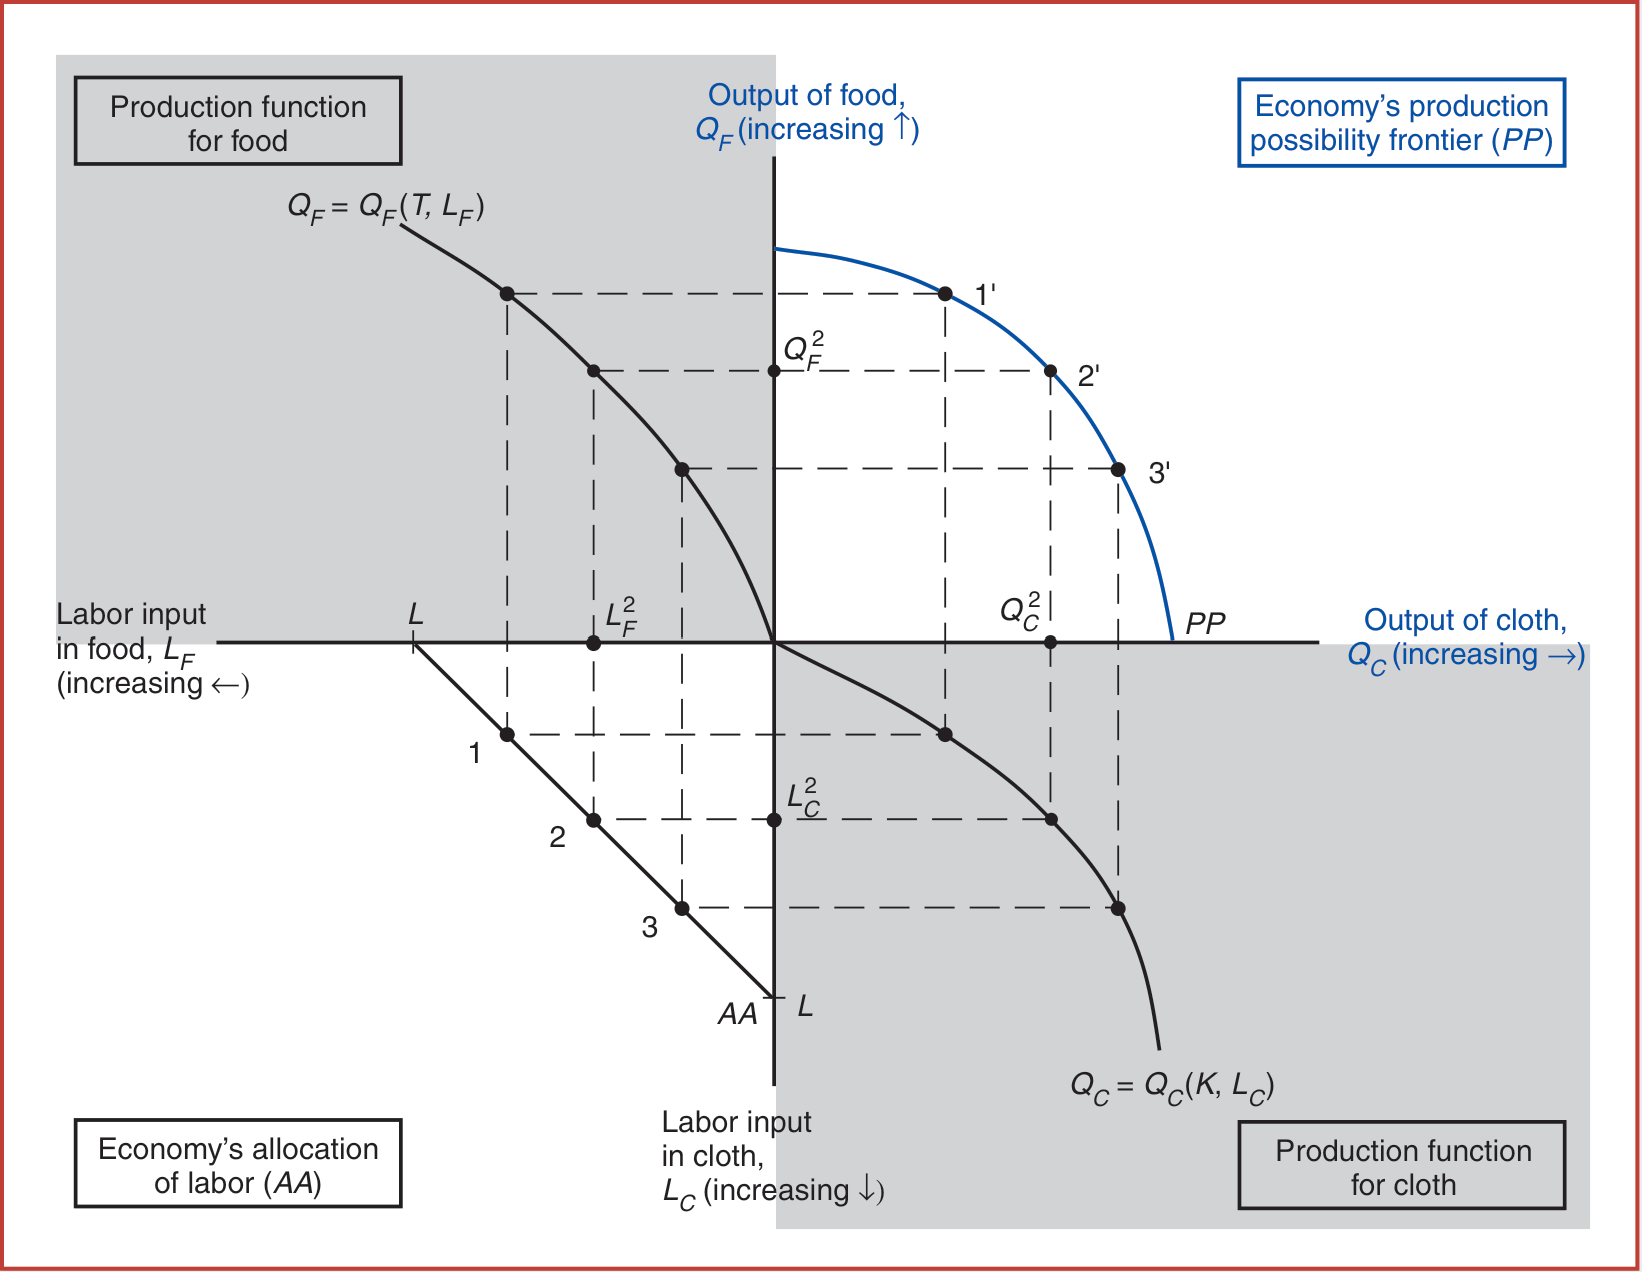
\includegraphics[width=0.8\textwidth]{figures/SFM_PPF.png}
    \caption{Production Possibility Frontier}
    \label{fig:lec4-1}
\end{figure}


Production of Good 1 and 2 is determined by the allocation of labor.
In the lower-left quadrant, the allocation between sectors can be illustrated by a point on line \textit{AA},
which represents all combinations of labor inupt of good 1 and 2 that sum up to total labor supplt $L$.

The curves in the lower-right and upper-left quadrants represent the production functions for both goods,
these allow determination of output $(Q_C^2, Q_F^2)$ given output.

\subsubsection{Gains from Trade}
Assume that the Home Country has a comparative advantage in good 1,
then $\frac{p_1}{p_2} < \left(\frac{p_1}{p_2}\right)^{ROW}$
\textcolor{red}{Waiting fro clarification}


\section{Richardo-Viner Model}
\label{sec:richardo-viner-model}

Consider an economy with two goods: $g=1,2$ and three factors of production: $L$, $K_1$, and $K_2$.

The output of good $g$ is given by:
\begin{gather*}
    y_g = f^g(L_g, K_g)
\end{gather*}
where $L_g$ is the endogenous amount of labor used in sector $g$ and $f^g$ is homogeneous of degree one in $(L_g, K_g)$.

\begin{remark}
    \begin{enumerate}
        \item $L$ is a ``mobile'' factor that can move between sectors.
        \item $K_1$ and $K_2$ are  ``immobile'' factors, can only be employed in one sector.
        \item Model is isomorphic to DRS model(\cite{dornbusch1977comparative}): $y_g = f^g(L_g)$ with $f_{LL}^g < 0$.
        \item Payments to specific factors under CRS is the same as profits under DRS.
    \end{enumerate}
\end{remark}

\subsection{Equilibrium: Small Open Economy}
We denote by $p_1$ and $p_2$ the prices of the two goods, and by $w$,
For now, as we are considering a small open economy, we will take $(p_1, p_2)$ as exogenously given.
So no need to look at good market clearing.

THe Profit Maximization Problem of the firm is given by:
\begin{gather*}
    \max_{L_g, K_g} \pi_g = p_g f^g(L_g, K_g) - wL_g - r_gK_g
\end{gather*}
so, the first order conditions are given by:
\begin{gather*}
    \frac{\partial \pi_g}{\partial L_g} = p_g f_{L}^g(L_g, K_g) - w = 0 \tag{1}\\
    \frac{\partial \pi_g}{\partial K_g} = p_g f_{K}^g(L_g, K_g) - r_g = 0 \tag{2}
\end{gather*}
The labor market clearing condition is given by:
\begin{gather*}
    L = L_1 + L_2 \tag{3}
\end{gather*}
Equations (1) and (3) jointly determine labor allocation and wage.

\subsection{Graphical Analysis}
At given prices and for a given endowment $K_g$, the Value of Marginal Product of Labor (VMPL) $p_g f_L^g(L_g, K_g)$ is the MPL curve
which is the demand curve of labor.

\tikzset{every picture/.style={line width=0.75pt}} %set default line width to 0.75pt        

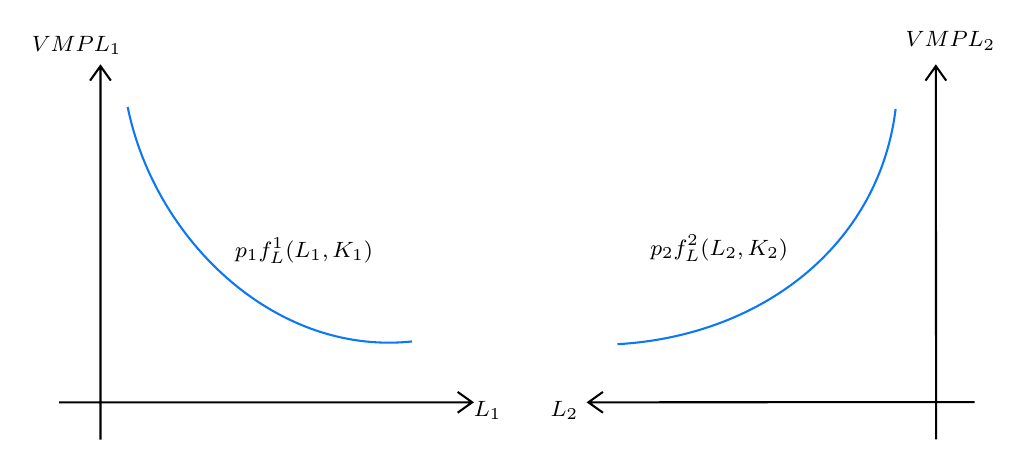
\begin{tikzpicture}[x=0.75pt,y=0.75pt,yscale=-1,xscale=1]
%uncomment if require: \path (0,300); %set diagram left start at 0, and has height of 300

%Shape: Axis 2D [id:dp0897128571489818] 
\draw  (50.67,212) -- (249.67,212)(70.57,50) -- (70.57,230) (242.67,207) -- (249.67,212) -- (242.67,217) (65.57,57) -- (70.57,50) -- (75.57,57)  ;
%Curve Lines [id:da9037261450642795] 
\draw [color={rgb, 255:red, 10; green, 119; blue, 247 }  ,draw opacity=1 ]   (83.67,69.67) .. controls (96.67,133.67) and (154.67,189.67) .. (220.67,182.67) ;
%Shape: Axis 2D [id:dp5550747519879127] 
\draw  (491.78,211.88) -- (305.65,212.01)(473.05,50.01) -- (473.18,229.88) (312.65,207.01) -- (305.65,212.01) -- (312.66,217.01) (478.06,57.01) -- (473.05,50.01) -- (468.06,57.02)  ;
%Curve Lines [id:da7136373564331845] 
\draw [color={rgb, 255:red, 10; green, 119; blue, 247 }  ,draw opacity=1 ]   (453.67,70.67) .. controls (445.67,136) and (389.67,180) .. (319.67,184) ;

% Text Node
\draw (134,131) node [anchor=north west][inner sep=0.75pt]  [font=\footnotesize] [align=left] {$\displaystyle p_{1} f_{L}^{1}( L_{1} ,K_{1})$};
% Text Node
\draw (249,210) node [anchor=north west][inner sep=0.75pt]  [font=\footnotesize] [align=left] {$\displaystyle L_{1}$};
% Text Node
\draw (36,34) node [anchor=north west][inner sep=0.75pt]  [font=\footnotesize] [align=left] {$\displaystyle VMPL_{1}$};
% Text Node
\draw (286,210) node [anchor=north west][inner sep=0.75pt]  [font=\footnotesize] [align=left] {$\displaystyle L_{2}$};
% Text Node
\draw (334,130) node [anchor=north west][inner sep=0.75pt]  [font=\footnotesize] [align=left] {$\displaystyle p_{2} f_{L}^{2}( L_{2} ,K_{2})$};
% Text Node
\draw (457,32) node [anchor=north west][inner sep=0.75pt]  [font=\footnotesize] [align=left] {$\displaystyle VMPL_{2}$};

\end{tikzpicture}

Combine the two VMPL curves for the two sectors


\tikzset{every picture/.style={line width=0.75pt}} %set default line width to 0.75pt        

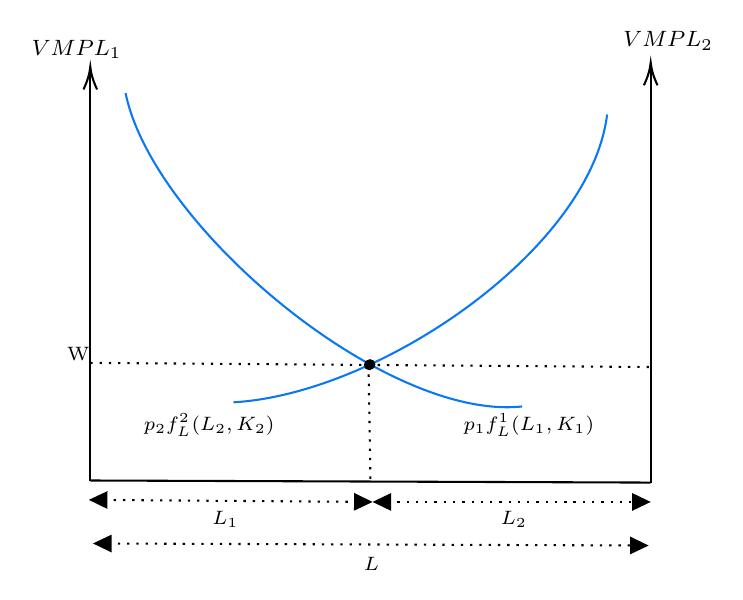
\begin{tikzpicture}[x=0.75pt,y=0.75pt,yscale=-1,xscale=1]
%uncomment if require: \path (0,300); %set diagram left start at 0, and has height of 300

%Straight Lines [id:da05723389757529007] 
\draw    (80.67,239.67) -- (80.67,42.33) ;
\draw [shift={(80.67,40.33)}, rotate = 90] [color={rgb, 255:red, 0; green, 0; blue, 0 }  ][line width=0.75]    (10.93,-3.29) .. controls (6.95,-1.4) and (3.31,-0.3) .. (0,0) .. controls (3.31,0.3) and (6.95,1.4) .. (10.93,3.29)   ;
%Straight Lines [id:da47485118019729256] 
\draw    (350.67,240.67) -- (350.67,40.33) ;
\draw [shift={(350.67,38.33)}, rotate = 90] [color={rgb, 255:red, 0; green, 0; blue, 0 }  ][line width=0.75]    (10.93,-3.29) .. controls (6.95,-1.4) and (3.31,-0.3) .. (0,0) .. controls (3.31,0.3) and (6.95,1.4) .. (10.93,3.29)   ;
%Straight Lines [id:da4658812754436358] 
\draw    (80.67,239.67) -- (350.67,240.67) ;
%Curve Lines [id:da854126868121665] 
\draw [color={rgb, 255:red, 10; green, 119; blue, 247 }  ,draw opacity=1 ]   (97.67,53) .. controls (110.67,117) and (222.67,211) .. (288.67,204) ;
%Curve Lines [id:da25082346474441075] 
\draw [color={rgb, 255:red, 10; green, 119; blue, 247 }  ,draw opacity=1 ]   (329.67,63.33) .. controls (323.96,109.96) and (270.38,158.62) .. (214.72,184.12) .. controls (192.38,194.35) and (169.71,200.85) .. (149.67,202) ;
%Straight Lines [id:da3150062246982779] 
\draw  [dash pattern={on 0.84pt off 2.51pt}]  (83,249.02) -- (213.67,249.98) ;
\draw [shift={(216.67,250)}, rotate = 180.42] [fill={rgb, 255:red, 0; green, 0; blue, 0 }  ][line width=0.08]  [draw opacity=0] (8.93,-4.29) -- (0,0) -- (8.93,4.29) -- cycle    ;
\draw [shift={(80,249)}, rotate = 0.42] [fill={rgb, 255:red, 0; green, 0; blue, 0 }  ][line width=0.08]  [draw opacity=0] (8.93,-4.29) -- (0,0) -- (8.93,4.29) -- cycle    ;
%Straight Lines [id:da7028415881904047] 
\draw    (212.67,182) ;
%Straight Lines [id:da5014455123724334] 
\draw  [dash pattern={on 0.84pt off 2.51pt}]  (214.72,184.12) -- (215.07,205.01) -- (215.67,240.17) ;
%Straight Lines [id:da7039693129091152] 
\draw  [dash pattern={on 0.84pt off 2.51pt}]  (80.67,183) -- (350.67,185) ;
%Straight Lines [id:da4206233265398237] 
\draw  [dash pattern={on 0.84pt off 2.51pt}]  (219.67,250) -- (347.67,250) ;
\draw [shift={(350.67,250)}, rotate = 180] [fill={rgb, 255:red, 0; green, 0; blue, 0 }  ][line width=0.08]  [draw opacity=0] (8.93,-4.29) -- (0,0) -- (8.93,4.29) -- cycle    ;
\draw [shift={(216.67,250)}, rotate = 0] [fill={rgb, 255:red, 0; green, 0; blue, 0 }  ][line width=0.08]  [draw opacity=0] (8.93,-4.29) -- (0,0) -- (8.93,4.29) -- cycle    ;
%Straight Lines [id:da45503646526403496] 
\draw  [dash pattern={on 0.84pt off 2.51pt}]  (85,270.01) -- (346.67,270.99) ;
\draw [shift={(349.67,271)}, rotate = 180.21] [fill={rgb, 255:red, 0; green, 0; blue, 0 }  ][line width=0.08]  [draw opacity=0] (8.93,-4.29) -- (0,0) -- (8.93,4.29) -- cycle    ;
\draw [shift={(82,270)}, rotate = 0.21] [fill={rgb, 255:red, 0; green, 0; blue, 0 }  ][line width=0.08]  [draw opacity=0] (8.93,-4.29) -- (0,0) -- (8.93,4.29) -- cycle    ;

% Text Node
\draw (105,206) node [anchor=north west][inner sep=0.75pt]  [font=\scriptsize] [align=left] {$p_{2} f_{L}^{2}( L_{2} ,K_{2})$};
% Text Node
\draw (259,206) node [anchor=north west][inner sep=0.75pt]  [font=\scriptsize] [align=left] {$p_{1} f_{L}^{1}( L_{1} ,K_{1})$};
% Text Node
\draw (68,174) node [anchor=north west][inner sep=0.75pt]   [align=left] {{\scriptsize W}};
% Text Node
\draw (138,253) node [anchor=north west][inner sep=0.75pt]  [font=\scriptsize] [align=left] {$L_{1}$};
% Text Node
\draw (277,253) node [anchor=north west][inner sep=0.75pt]  [font=\scriptsize] [align=left] {$L_{2}$};
% Text Node
\draw (211,275) node [anchor=north west][inner sep=0.75pt]  [font=\scriptsize] [align=left] {$L$};
% Text Node
\draw (51,26) node [anchor=north west][inner sep=0.75pt]  [font=\footnotesize] [align=left] {$VMPL_{1}$};
% Text Node
\draw (336,22) node [anchor=north west][inner sep=0.75pt]  [font=\footnotesize] [align=left] {$VMPL_{2}$};

\draw [fill={rgb, 255:red, 0; green, 0; blue, 0 }  ,fill opacity=1 ]  (215.51, 183.75) circle [x radius= 2, y radius= 2]   ;
\draw [fill={rgb, 255:red, 0; green, 0; blue, 0 }  ,fill opacity=1 ]  (214.99, 183.99) circle [x radius= 2, y radius= 2]   ;
\end{tikzpicture}

The horizontal axis measures $L$: i.e., full employment.
Intersection of two demand curves determines equilibrium wage
and allocation of labor between sectors

Equilibrium payments to the specific factors are given by:
\begin{gather*}
    K_g r_g = \int_{0}^{L_g} \left(p_g f_L^g(L, K_g) - w \right) \, dL_g
\end{gather*}

\subsection{Comparative Statics}
\subsubsection{TOT shock}
Suppose the economy experiences a TOT shock such that $p_1$ increases,

\tikzset{every picture/.style={line width=0.75pt}} %set default line width to 0.75pt        

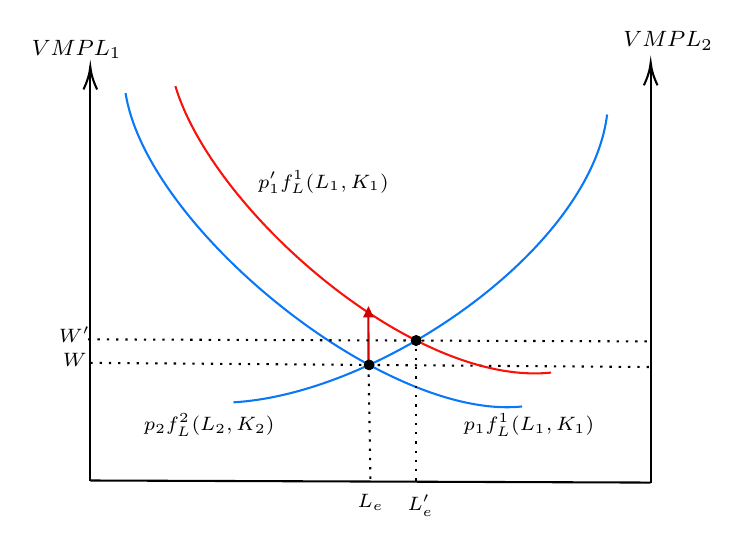
\begin{tikzpicture}[x=0.75pt,y=0.75pt,yscale=-1,xscale=1]
%uncomment if require: \path (0,300); %set diagram left start at 0, and has height of 300

%Straight Lines [id:da07752523780951825] 
\draw    (80.67,239.67) -- (80.67,42.33) ;
\draw [shift={(80.67,40.33)}, rotate = 90] [color={rgb, 255:red, 0; green, 0; blue, 0 }  ][line width=0.75]    (10.93,-3.29) .. controls (6.95,-1.4) and (3.31,-0.3) .. (0,0) .. controls (3.31,0.3) and (6.95,1.4) .. (10.93,3.29)   ;
%Straight Lines [id:da7181686746748042] 
\draw    (350.67,240.67) -- (350.67,40.33) ;
\draw [shift={(350.67,38.33)}, rotate = 90] [color={rgb, 255:red, 0; green, 0; blue, 0 }  ][line width=0.75]    (10.93,-3.29) .. controls (6.95,-1.4) and (3.31,-0.3) .. (0,0) .. controls (3.31,0.3) and (6.95,1.4) .. (10.93,3.29)   ;
%Straight Lines [id:da4325450410729055] 
\draw    (80.67,239.67) -- (350.67,240.67) ;
%Curve Lines [id:da9822178045586689] 
\draw [color={rgb, 255:red, 10; green, 119; blue, 247 }  ,draw opacity=1 ]   (97.67,53) .. controls (107.67,117.67) and (222.67,211) .. (288.67,204) ;
%Curve Lines [id:da791078015837639] 
\draw [color={rgb, 255:red, 10; green, 119; blue, 247 }  ,draw opacity=1 ]   (329.67,63.33) .. controls (323.96,109.96) and (270.38,158.62) .. (214.72,184.12) .. controls (192.38,194.35) and (169.71,200.85) .. (149.67,202) ;
%Straight Lines [id:da08255683624142351] 
\draw    (212.67,182) ;
%Straight Lines [id:da3379661384304282] 
\draw  [dash pattern={on 0.84pt off 2.51pt}]  (214.72,184.12) -- (215.07,205.01) -- (215.67,240.17) ;
%Straight Lines [id:da05152562939913974] 
\draw  [dash pattern={on 0.84pt off 2.51pt}]  (80.67,183) -- (350.67,185) ;
%Curve Lines [id:da1534055140915196] 
\draw [color={rgb, 255:red, 247; green, 18; blue, 10 }  ,draw opacity=1 ]   (121.67,49.67) .. controls (139.67,109.67) and (236.67,194.67) .. (302.67,187.67) ;
%Straight Lines [id:da11656998235372307] 
\draw [color={rgb, 255:red, 208; green, 2; blue, 2 }  ,draw opacity=1 ]   (214.72,184.12) -- (214.67,158.67) ;
\draw [shift={(214.67,155.67)}, rotate = 89.89] [fill={rgb, 255:red, 208; green, 2; blue, 2 }  ,fill opacity=1 ][line width=0.08]  [draw opacity=0] (5.36,-2.57) -- (0,0) -- (5.36,2.57) -- cycle    ;
%Straight Lines [id:da24481276852593314] 
\draw  [dash pattern={on 0.84pt off 2.51pt}]  (79.67,171.67) -- (350.67,172.67) ;
%Straight Lines [id:da7254070417172829] 
\draw  [dash pattern={on 0.84pt off 2.51pt}]  (237.67,171.67) -- (237.67,240.67) ;

% Text Node
\draw (105,206) node [anchor=north west][inner sep=0.75pt]  [font=\scriptsize] [align=left] {$p_{2} f_{L}^{2}( L_{2} ,K_{2})$};
% Text Node
\draw (259,206) node [anchor=north west][inner sep=0.75pt]  [font=\scriptsize] [align=left] {$p_{1} f_{L}^{1}( L_{1} ,K_{1})$};
% Text Node
\draw (66,177) node [anchor=north west][inner sep=0.75pt]  [font=\footnotesize] [align=left] {{\scriptsize $W$}};
% Text Node
\draw (208,245) node [anchor=north west][inner sep=0.75pt]  [font=\scriptsize] [align=left] {$L_{e}$};
% Text Node
\draw (232,245) node [anchor=north west][inner sep=0.75pt]  [font=\scriptsize] [align=left] {$L_{e}^{\prime} $};
% Text Node
\draw (51,26) node [anchor=north west][inner sep=0.75pt]  [font=\footnotesize] [align=left] {$VMPL_{1}$};
% Text Node
\draw (336,22) node [anchor=north west][inner sep=0.75pt]  [font=\footnotesize] [align=left] {$VMPL_{2}$};
% Text Node
\draw (64,164) node [anchor=north west][inner sep=0.75pt]  [font=\footnotesize] [align=left] {{\scriptsize $W^{\prime}$}};
% Text Node
\draw (160,89) node [anchor=north west][inner sep=0.75pt]  [font=\scriptsize] [align=left] {$p_{1}^{\prime} f_{L}^{1}( L_{1} ,K_{1})$};

\draw [fill={rgb, 255:red, 0; green, 0; blue, 0 }  ,fill opacity=1 ]  (215.03, 183.98) circle [x radius= 2, y radius= 2]   ;
\draw [fill={rgb, 255:red, 0; green, 0; blue, 0 }  ,fill opacity=1 ]  (214.99, 183.99) circle [x radius= 2, y radius= 2]   ;
\draw [fill={rgb, 255:red, 0; green, 0; blue, 0 }  ,fill opacity=1 ]  (237.7, 172.2) circle [x radius= 2, y radius= 2]   ;
\draw [fill={rgb, 255:red, 0; green, 0; blue, 0 }  ,fill opacity=1 ]  (237.62, 172.25) circle [x radius= 2, y radius= 2]   ;
\draw [fill={rgb, 255:red, 0; green, 0; blue, 0 }  ,fill opacity=1 ]  (237.67, 172.22) circle [x radius= 2, y radius= 2]   ;
\end{tikzpicture}

Then the labor demand curve for good 1 shifts to the right, the labor demand in sector 1 $L_1$ increases,
as the tal labor supply is fixed, the labor demand in sector 2 $L_2$ decreases.

As $y \propto L$, $L_1$ increases gives us that $y_1$ increases, and $y_2$ decreases.
From the graph, we can also tell that the wage increases, but, the wage-price ratio $w/p_1$ decreases:
\begin{gather*}
    \frac{d w}{d p_1} = f_L^1 + p_1 f_{LL}^1 \frac{d L_1}{d p_1} < f_L^1 = \frac{w}{p_1}
\end{gather*}
So, 
\begin{gather*}
    \frac{dw}{w} = \hat{w} < \hat{p_1} = \frac{dp_1}{p_1}
\end{gather*}
Condition (2) gives us that:
\begin{gather*}
    \frac{d r_1}{d p_1} = f_K^1 + p_1 f_{KL}^{1} \frac{d L_1}{d p_1} > f_K^1 = \frac{r_1}{p_1} \Rightarrow \hat{r_1} > \hat{p_1} \\
    r_2, \text{ and a fortiori } \frac{r_2}{p_1} \downarrow
\end{gather*}

\begin{theorem}[Magnification effect]
    \

    Assuming that $\hat{p_2} < \hat{p_1}$, then:
    \begin{gather*}
        \hat{r_2} < \hat{p_2} < \hat{w} < \hat{p_1} < \hat{r_1}
    \end{gather*}
\end{theorem}

We can use the same type of arguments to analyze consequences of:
\begin{itemize}
    \item Productivity shocks
    \item Changes in factor endowments
\end{itemize}

\subsubsection{Effect of an increase in $L$:}
In this case, we have:
\begin{itemize}
    \item $L_1 \uparrow$, $L_2 \downarrow$;
    \item $y_1 \uparrow$, $y_2 \downarrow$;
    \item $w \downarrow$;
    \item $r_1 \uparrow$; $r_2 \uparrow$.
\end{itemize}

\tikzset{every picture/.style={line width=0.75pt}} %set default line width to 0.75pt        

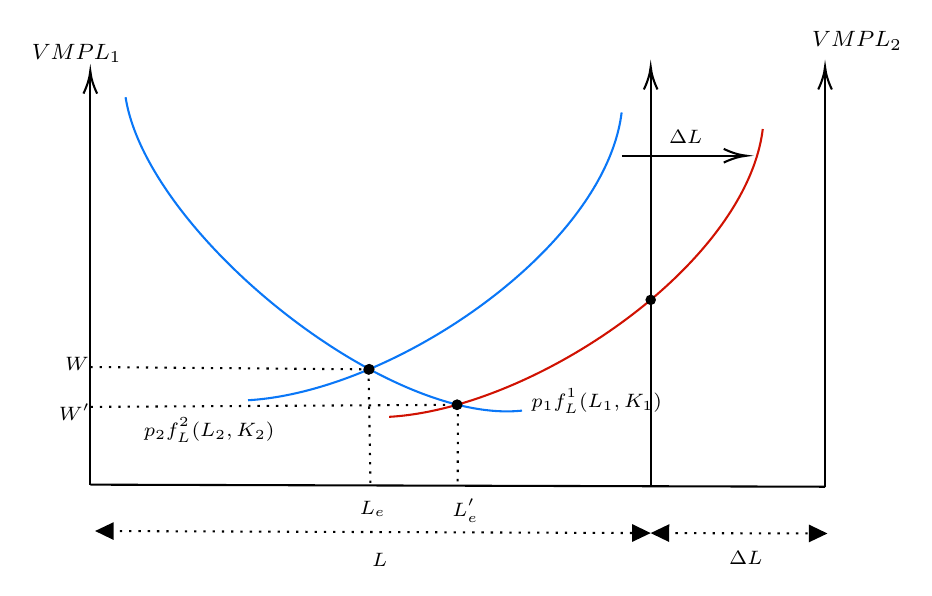
\begin{tikzpicture}[x=0.75pt,y=0.75pt,yscale=-1,xscale=1]
%uncomment if require: \path (0,300); %set diagram left start at 0, and has height of 300

%Straight Lines [id:da9207501752825712] 
\draw    (80.67,239.67) -- (80.67,42.33) ;
\draw [shift={(80.67,40.33)}, rotate = 90] [color={rgb, 255:red, 0; green, 0; blue, 0 }  ][line width=0.75]    (10.93,-3.29) .. controls (6.95,-1.4) and (3.31,-0.3) .. (0,0) .. controls (3.31,0.3) and (6.95,1.4) .. (10.93,3.29)   ;
%Straight Lines [id:da39783234243981513] 
\draw    (350.67,240.67) -- (350.67,40.33) ;
\draw [shift={(350.67,38.33)}, rotate = 90] [color={rgb, 255:red, 0; green, 0; blue, 0 }  ][line width=0.75]    (10.93,-3.29) .. controls (6.95,-1.4) and (3.31,-0.3) .. (0,0) .. controls (3.31,0.3) and (6.95,1.4) .. (10.93,3.29)   ;
%Straight Lines [id:da04788118702647359] 
\draw    (80.67,239.67) -- (434.67,240.67) ;
%Curve Lines [id:da11924022022699887] 
\draw [color={rgb, 255:red, 10; green, 119; blue, 247 }  ,draw opacity=1 ]   (97.67,53) .. controls (107.67,117.67) and (222.67,211) .. (288.67,204) ;
%Curve Lines [id:da22841932286757227] 
\draw [color={rgb, 255:red, 10; green, 119; blue, 247 }  ,draw opacity=1 ]   (336.67,60.33) .. controls (330.96,106.96) and (277.38,155.62) .. (221.72,181.12) .. controls (199.38,191.35) and (176.71,197.85) .. (156.67,199) ;
%Straight Lines [id:da8766667566126164] 
\draw    (212.67,182) ;
%Straight Lines [id:da615626010835146] 
\draw  [dash pattern={on 0.84pt off 2.51pt}]  (214.72,184.12) -- (215.07,205.01) -- (215.67,240.17) ;
%Straight Lines [id:da7823333394231944] 
\draw  [dash pattern={on 0.84pt off 2.51pt}]  (80.67,183) -- (214.72,184.12) ;
%Straight Lines [id:da9476268980386685] 
\draw    (434.67,240.67) -- (434.67,40.33) ;
\draw [shift={(434.67,38.33)}, rotate = 90] [color={rgb, 255:red, 0; green, 0; blue, 0 }  ][line width=0.75]    (10.93,-3.29) .. controls (6.95,-1.4) and (3.31,-0.3) .. (0,0) .. controls (3.31,0.3) and (6.95,1.4) .. (10.93,3.29)   ;
%Curve Lines [id:da9819804107733794] 
\draw [color={rgb, 255:red, 208; green, 18; blue, 2 }  ,draw opacity=1 ]   (404.67,68.33) .. controls (398.96,114.96) and (345.38,163.62) .. (289.72,189.12) .. controls (267.38,199.35) and (244.71,205.85) .. (224.67,207) ;
%Straight Lines [id:da3948413936785935] 
\draw    (336.8,81.2) -- (394.8,81.2) ;
\draw [shift={(396.8,81.2)}, rotate = 180] [color={rgb, 255:red, 0; green, 0; blue, 0 }  ][line width=0.75]    (10.93,-3.29) .. controls (6.95,-1.4) and (3.31,-0.3) .. (0,0) .. controls (3.31,0.3) and (6.95,1.4) .. (10.93,3.29)   ;
%Straight Lines [id:da8643271498154601] 
\draw  [dash pattern={on 0.84pt off 2.51pt}]  (80.8,202.2) -- (257.8,201.2) ;
%Straight Lines [id:da6127658964549799] 
\draw  [dash pattern={on 0.84pt off 2.51pt}]  (257.8,201.2) -- (257.67,240.17) ;
%Straight Lines [id:da12380375901271923] 
\draw  [dash pattern={on 0.84pt off 2.51pt}]  (86,262.01) -- (347.67,262.99) ;
\draw [shift={(350.67,263)}, rotate = 180.21] [fill={rgb, 255:red, 0; green, 0; blue, 0 }  ][line width=0.08]  [draw opacity=0] (8.93,-4.29) -- (0,0) -- (8.93,4.29) -- cycle    ;
\draw [shift={(83,262)}, rotate = 0.21] [fill={rgb, 255:red, 0; green, 0; blue, 0 }  ][line width=0.08]  [draw opacity=0] (8.93,-4.29) -- (0,0) -- (8.93,4.29) -- cycle    ;
%Straight Lines [id:da4119464555704524] 
\draw  [dash pattern={on 0.84pt off 2.51pt}]  (353.67,263.01) -- (432.8,263.19) ;
\draw [shift={(435.8,263.2)}, rotate = 180.13] [fill={rgb, 255:red, 0; green, 0; blue, 0 }  ][line width=0.08]  [draw opacity=0] (8.93,-4.29) -- (0,0) -- (8.93,4.29) -- cycle    ;
\draw [shift={(350.67,263)}, rotate = 0.13] [fill={rgb, 255:red, 0; green, 0; blue, 0 }  ][line width=0.08]  [draw opacity=0] (8.93,-4.29) -- (0,0) -- (8.93,4.29) -- cycle    ;

% Text Node
\draw (105,206) node [anchor=north west][inner sep=0.75pt]  [font=\scriptsize] [align=left] {$\displaystyle p_{2} f_{L}^{2}( L_{2} ,K_{2})$};
% Text Node
\draw (291.72,192.12) node [anchor=north west][inner sep=0.75pt]  [font=\scriptsize] [align=left] {$\displaystyle p_{1} f_{L}^{1}( L_{1} ,K_{1})$};
% Text Node
\draw (67,177) node [anchor=north west][inner sep=0.75pt]  [font=\footnotesize] [align=left] {{\scriptsize $\displaystyle W$}};
% Text Node
\draw (209,246) node [anchor=north west][inner sep=0.75pt]  [font=\scriptsize] [align=left] {$\displaystyle L_{e}$};
% Text Node
\draw (253.67,245.17) node [anchor=north west][inner sep=0.75pt]  [font=\scriptsize] [align=left] {$\displaystyle L'_{e}$};
% Text Node
\draw (51,26) node [anchor=north west][inner sep=0.75pt]  [font=\footnotesize] [align=left] {$\displaystyle VMPL_{1}$};
% Text Node
\draw (427,20) node [anchor=north west][inner sep=0.75pt]  [font=\footnotesize] [align=left] {$\displaystyle VMPL_{2}$};
% Text Node
\draw (64,199) node [anchor=north west][inner sep=0.75pt]  [font=\footnotesize] [align=left] {{\scriptsize $\displaystyle W'$}};
% Text Node
\draw (358,67.4) node [anchor=north west][inner sep=0.75pt]  [font=\scriptsize]  {$\Delta L$};
% Text Node
\draw (215,271) node [anchor=north west][inner sep=0.75pt]  [font=\scriptsize] [align=left] {$\displaystyle L$};
% Text Node
\draw (387,270.4) node [anchor=north west][inner sep=0.75pt]  [font=\scriptsize]  {$\Delta L$};

\draw [fill={rgb, 255:red, 0; green, 0; blue, 0 }  ,fill opacity=1 ]  (215.12, 184.03) circle [x radius= 2, y radius= 2]   ;
\draw [fill={rgb, 255:red, 0; green, 0; blue, 0 }  ,fill opacity=1 ]  (214.72, 184.2) circle [x radius= 2, y radius= 2]   ;
\draw [fill={rgb, 255:red, 0; green, 0; blue, 0 }  ,fill opacity=1 ]  (350.67, 150.64) circle [x radius= 2, y radius= 2]   ;
\draw [fill={rgb, 255:red, 0; green, 0; blue, 0 }  ,fill opacity=1 ]  (257.48, 201.15) circle [x radius= 2, y radius= 2]   ;
\draw [fill={rgb, 255:red, 0; green, 0; blue, 0 }  ,fill opacity=1 ]  (257.27, 201.2) circle [x radius= 2, y radius= 2]   ;
\end{tikzpicture}


\subsubsection{Effect of an increase in $K_1$:}
In this case, we have:
\begin{itemize}
    \item $L_1 \uparrow$, $L_2 \downarrow$;
    \item $y_1 \uparrow$, $y_2 \downarrow$;
    \item $w \uparrow$;
    \item $r_1 \downarrow$; $r_2 \downarrow$.
\end{itemize}



\tikzset{every picture/.style={line width=0.75pt}} %set default line width to 0.75pt        

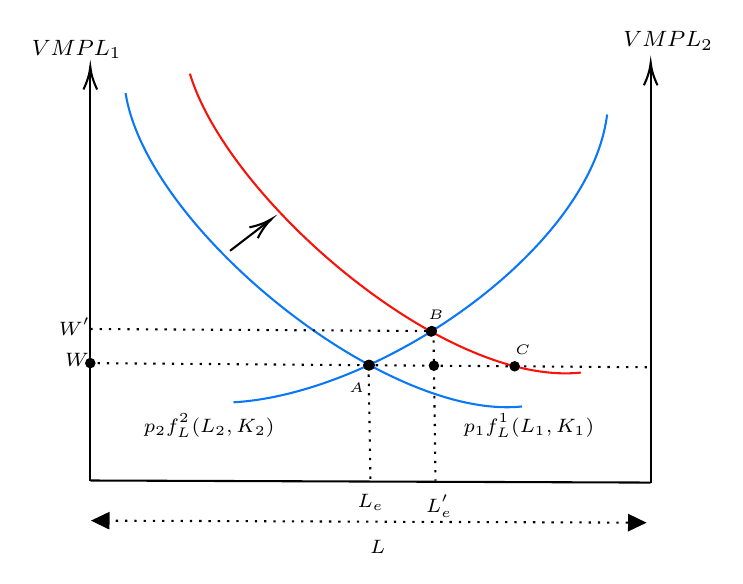
\begin{tikzpicture}[x=0.75pt,y=0.75pt,yscale=-1,xscale=1]
%uncomment if require: \path (0,300); %set diagram left start at 0, and has height of 300

%Straight Lines [id:da3185353693601837] 
\draw    (80.67,239.67) -- (80.67,42.33) ;
\draw [shift={(80.67,40.33)}, rotate = 90] [color={rgb, 255:red, 0; green, 0; blue, 0 }  ][line width=0.75]    (10.93,-3.29) .. controls (6.95,-1.4) and (3.31,-0.3) .. (0,0) .. controls (3.31,0.3) and (6.95,1.4) .. (10.93,3.29)   ;
%Straight Lines [id:da33810683987776036] 
\draw    (350.67,240.67) -- (350.67,40.33) ;
\draw [shift={(350.67,38.33)}, rotate = 90] [color={rgb, 255:red, 0; green, 0; blue, 0 }  ][line width=0.75]    (10.93,-3.29) .. controls (6.95,-1.4) and (3.31,-0.3) .. (0,0) .. controls (3.31,0.3) and (6.95,1.4) .. (10.93,3.29)   ;
%Straight Lines [id:da7144825094982482] 
\draw    (80.67,239.67) -- (350.67,240.67) ;
%Curve Lines [id:da10515844568295973] 
\draw [color={rgb, 255:red, 10; green, 119; blue, 247 }  ,draw opacity=1 ]   (97.67,53) .. controls (107.67,117.67) and (222.67,211) .. (288.67,204) ;
%Curve Lines [id:da16182226195544724] 
\draw [color={rgb, 255:red, 10; green, 119; blue, 247 }  ,draw opacity=1 ]   (329.67,63.33) .. controls (323.96,109.96) and (270.38,158.62) .. (214.72,184.12) .. controls (192.38,194.35) and (169.71,200.85) .. (149.67,202) ;
%Straight Lines [id:da7128499178139281] 
\draw    (212.67,182) ;
%Straight Lines [id:da3562087733885887] 
\draw  [dash pattern={on 0.84pt off 2.51pt}]  (214.72,184.12) -- (215.07,205.01) -- (215.67,240.17) ;
%Straight Lines [id:da49374956785143154] 
\draw  [dash pattern={on 0.84pt off 2.51pt}]  (79.72,183.12) -- (349.72,185.12) ;
%Curve Lines [id:da07835712346608026] 
\draw [color={rgb, 255:red, 247; green, 18; blue, 10 }  ,draw opacity=1 ]   (128.67,43.67) .. controls (146.67,103.67) and (251,194.67) .. (317,187.67) ;
%Straight Lines [id:da8151273642018261] 
\draw  [dash pattern={on 0.84pt off 2.51pt}]  (80.67,166.67) -- (246,167.67) ;
%Straight Lines [id:da17058966404454246] 
\draw  [dash pattern={on 0.84pt off 2.51pt}]  (246,167.67) -- (247,239.67) ;
%Straight Lines [id:da5409712805527545] 
\draw    (148,129) -- (166.41,114.88) ;
\draw [shift={(168,113.67)}, rotate = 142.52] [color={rgb, 255:red, 0; green, 0; blue, 0 }  ][line width=0.75]    (10.93,-3.29) .. controls (6.95,-1.4) and (3.31,-0.3) .. (0,0) .. controls (3.31,0.3) and (6.95,1.4) .. (10.93,3.29)   ;
%Straight Lines [id:da5407251933426643] 
\draw  [dash pattern={on 0.84pt off 2.51pt}]  (84,259.01) -- (345.67,259.99) ;
\draw [shift={(348.67,260)}, rotate = 180.21] [fill={rgb, 255:red, 0; green, 0; blue, 0 }  ][line width=0.08]  [draw opacity=0] (8.93,-4.29) -- (0,0) -- (8.93,4.29) -- cycle    ;
\draw [shift={(81,259)}, rotate = 0.21] [fill={rgb, 255:red, 0; green, 0; blue, 0 }  ][line width=0.08]  [draw opacity=0] (8.93,-4.29) -- (0,0) -- (8.93,4.29) -- cycle    ;

% Text Node
\draw (105,206) node [anchor=north west][inner sep=0.75pt]  [font=\scriptsize] [align=left] {$\displaystyle p_{2} f_{L}^{2}( L_{2} ,K_{2})$};
% Text Node
\draw (259,206) node [anchor=north west][inner sep=0.75pt]  [font=\scriptsize] [align=left] {$\displaystyle p_{1} f_{L}^{1}( L_{1} ,K_{1})$};
% Text Node
\draw (67,177) node [anchor=north west][inner sep=0.75pt]  [font=\footnotesize] [align=left] {{\scriptsize $\displaystyle W$}};
% Text Node
\draw (208,245) node [anchor=north west][inner sep=0.75pt]  [font=\scriptsize] [align=left] {$\displaystyle L_{e}$};
% Text Node
\draw (241,245) node [anchor=north west][inner sep=0.75pt]  [font=\scriptsize] [align=left] {$\displaystyle L'_{e}$};
% Text Node
\draw (51,26) node [anchor=north west][inner sep=0.75pt]  [font=\footnotesize] [align=left] {$\displaystyle VMPL_{1}$};
% Text Node
\draw (336,22) node [anchor=north west][inner sep=0.75pt]  [font=\footnotesize] [align=left] {$\displaystyle VMPL_{2}$};
% Text Node
\draw (64,160) node [anchor=north west][inner sep=0.75pt]  [font=\footnotesize] [align=left] {{\scriptsize $\displaystyle W'$}};
% Text Node
\draw (204,191) node [anchor=north west][inner sep=0.75pt]  [font=\tiny] [align=left] {$\displaystyle A$};
% Text Node
\draw (242,156) node [anchor=north west][inner sep=0.75pt]  [font=\tiny] [align=left] {$\displaystyle B$};
% Text Node
\draw (284,173) node [anchor=north west][inner sep=0.75pt]  [font=\tiny] [align=left] {$\displaystyle C$};
% Text Node
\draw (214,267) node [anchor=north west][inner sep=0.75pt]  [font=\scriptsize] [align=left] {$\displaystyle L$};

\draw [fill={rgb, 255:red, 0; green, 0; blue, 0 }  ,fill opacity=1 ]  (215.03, 183.98) circle [x radius= 2, y radius= 2]   ;
\draw [fill={rgb, 255:red, 0; green, 0; blue, 0 }  ,fill opacity=1 ]  (214.72, 184.12) circle [x radius= 2, y radius= 2]   ;
\draw [fill={rgb, 255:red, 0; green, 0; blue, 0 }  ,fill opacity=1 ]  (214.72, 184.12) circle [x radius= 2, y radius= 2]   ;
\draw [fill={rgb, 255:red, 0; green, 0; blue, 0 }  ,fill opacity=1 ]  (244.85, 167.9) circle [x radius= 2, y radius= 2]   ;
\draw [fill={rgb, 255:red, 0; green, 0; blue, 0 }  ,fill opacity=1 ]  (245.24, 167.66) circle [x radius= 2, y radius= 2]   ;
\draw [fill={rgb, 255:red, 0; green, 0; blue, 0 }  ,fill opacity=1 ]  (80.67, 183.12) circle [x radius= 2, y radius= 2]   ;
\draw [fill={rgb, 255:red, 0; green, 0; blue, 0 }  ,fill opacity=1 ]  (215.29, 184.12) circle [x radius= 2, y radius= 2]   ;
\draw [fill={rgb, 255:red, 0; green, 0; blue, 0 }  ,fill opacity=1 ]  (214.72, 184.12) circle [x radius= 2, y radius= 2]   ;
\draw [fill={rgb, 255:red, 0; green, 0; blue, 0 }  ,fill opacity=1 ]  (285.14, 184.64) circle [x radius= 2, y radius= 2]   ;
\draw [fill={rgb, 255:red, 0; green, 0; blue, 0 }  ,fill opacity=1 ]  (246.23, 184.35) circle [x radius= 2, y radius= 2]   ;
\end{tikzpicture}

\begin{note}
    \

    In all cases, results are intuitive:
    \begin{itemize}
        \item ``Dutch disease'' (Boom in export sectors, Bids up wages, which
        leads to a contraction in the other sectors)
        \item Useful political-economy applications (Grossman and Helpman
        1994)
    \end{itemize}

    It's also easy to extend the analysis to more than 2 sectors:
    \begin{itemize}
        \item Plot labor demand in one sector vs. rest of the economy
        \item Convenient for empirical work (Kovak 2013)
    \end{itemize}
\end{note}

\subsection{Equilibrium: Two-country World}

Predictions on the pattern of trade in a two-country world depend on
whether differences in factor endowments come from:
\begin{itemize}
    \item Differences in the relative supply of specific factors
    \item Differences in the relative supply of mobile factors
\end{itemize}
Accordingly, any change in factor prices is possible as we move from
autarky to free trade (see Feenstra Problem 3.1 p. 98)

\subsection{Concluding remarks on Ricardo-Viner Model}
In Ricardo's model, if the two countries had identical technologies,
there would be no difference in autarkic relative prices, so no
comparative advantage and no reason to trade.

In the Ricardo-Viner model, even if the two countries have identical
technologies (same production functions $f^1(., .)$, $f^2(., .)$),
their factor endowment differences can create comparative advantage.

In Ricardo, trade can lead to complete specialization:
import-competing sector disappears completely.

In Ricardo-Viner, this cannot happen. If all labor were to leave the sector 1,
the marginal product of labor there, working with the given fixed
$K_1$, would be very high. So it would be profitable / efficient to bring
back some labor into 1. Efficiency / equilibrium condition is
equality of values of marginal products.

In Ricardo there was no distributional conflict. In Specific Factors
there is very sharp distributional conflict between owners of the
specific capital in the two sectors. Workers may side with either;
depends on their consumption pattern.

\subsection{General Conclusions for Ricardo-Viner Model}

The differences in recourses is a source of comparative advantage, and in trade, there are both winners and losers.
Winners are factors specific to export sectors;
losers are factors specific to import-competing sectors.

Winners could compensate losers, but in practice,
such compensation is rarely carried out fully.
Though there are examples of partial compensation (e.g.,
adjustment assistance, retraining subsidies, temporary
subsidies...)

\subsection{Political Economy of Trade}

countries gain overall form trade, but distributional conflict. Then, should trade be restricted?
Few economists would agree.

The income distribution effects are not specific to international trade, it could also due to technological progress, etc.
Why trade effects of trade differently?
